% Created 2024-08-31 Sat 13:55
% Intended LaTeX compiler: pdflatex
\documentclass[11pt]{article}
\usepackage[utf8]{inputenc}
\usepackage[T1]{fontenc}
\usepackage{graphicx}
\usepackage{longtable}
\usepackage{wrapfig}
\usepackage{rotating}
\usepackage[normalem]{ulem}
\usepackage{amsmath}
\usepackage{amssymb}
\usepackage{capt-of}
\usepackage{hyperref}
\author{Rohan Jeendgar}
\date{\today}
\title{L1}
\hypersetup{
 pdfauthor={Rohan Jeendgar},
 pdftitle={L1},
 pdfkeywords={},
 pdfsubject={},
 pdfcreator={Emacs 29.4 (Org mode 9.8)}, 
 pdflang={English}}
\begin{document}

\maketitle
\tableofcontents

\section{Questions}
\label{sec:org73bb228}
\subsection{Q1 - Sample}
\label{sec:orgb26f742}
\subsection{Q2 - Find all the 12" Vinyl releases of the Beatles in the United Kingdoms up until the year they broke up.}
\label{sec:orgc401736}
\subsubsection{Query}
\label{sec:orgabeb225}
\begin{verbatim}
SELECT
    distinct(r.name) AS album_name,
    ri.date_year AS release_year
FROM
    release r
JOIN
    artist_credit ac ON r.artist_credit = ac.id
JOIN
    artist a ON ac.id = a.id
JOIN
    medium m ON r.id = m.release
JOIN
    medium_format mf ON m.format = mf.id
JOIN
    release_info ri ON r.id = ri.release
JOIN
    area ar ON ri.area = ar.id
WHERE
    a.name = 'The Beatles'
    AND mf.name = '12" Vinyl'
    AND ar.name = 'United Kingdom'
    AND ri.date_year <= 1970
ORDER BY
    ri.date_year ASC;

\end{verbatim}
\subsubsection{Output}
\label{sec:orgeb330e0}
\begin{center}
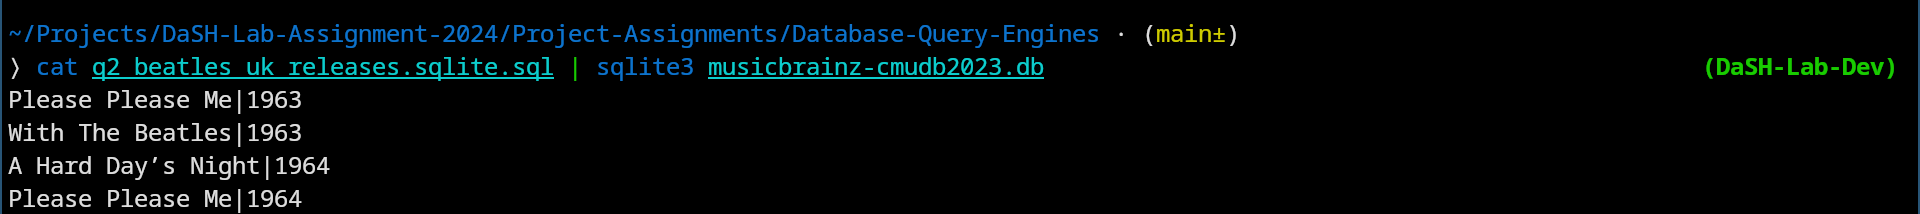
\includegraphics[width=.9\linewidth]{./images/Q2.png}
\end{center}
\subsection{Q3 - Find the ten newest release that has the medium format Cassette.}
\label{sec:orgc443dda}
\subsubsection{Query}
\label{sec:org83974b6}
\begin{verbatim}
SELECT
    r.name AS release_name,
    ac.name AS artist_name,
    ri.date_year AS release_year
FROM
    release r
JOIN
    artist_credit ac ON r.artist_credit = ac.id
JOIN
    release_info ri ON r.id = ri.release
JOIN
    medium me ON r.id = me.release
JOIN
    medium_format mf ON me.format = mf.id
WHERE
    mf.name LIKE 'Cassette'
ORDER BY
    ri.date_year DESC,
    ri.date_month DESC,
    ri.date_day DESC,
    r.name ASC,
    ac.name ASC
LIMIT 10;

\end{verbatim}
\subsubsection{Output}
\label{sec:orga536439}
\begin{center}
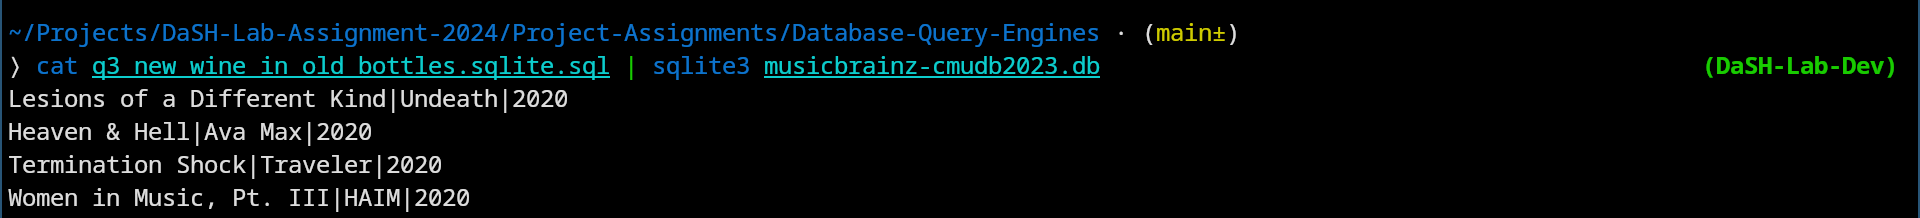
\includegraphics[width=.9\linewidth]{./images/Q3.png}
\end{center}
\subsection{Q4 - Find works with the longest comment for each work type.}
\label{sec:org49b3a9b}
\subsubsection{Query}
\label{sec:orgceb0db2}
\begin{verbatim}
 SELECT
    distinct(wt.name) AS WORK_TYPE,
    w.name AS WORK_NAME,
    LENGTH(w.comment) AS COMMENT_LENGTH,
    w.comment as 'COMMENT'
FROM
    work w
JOIN
    work_type wt ON w.type = wt.id
JOIN
    (
        SELECT
            type,
            MAX(LENGTH(comment)) AS max_comment_length
        FROM
            work
        WHERE
            LENGTH(comment) > 0
        GROUP BY
            type
    ) max_comments ON w.type = max_comments.type
                  AND LENGTH(w.comment) = max_comments.max_comment_length
ORDER BY
    wt.name ASC,
    w.name ASC;
\end{verbatim}
\subsubsection{Output}
\label{sec:orged4ffdd}
\begin{center}
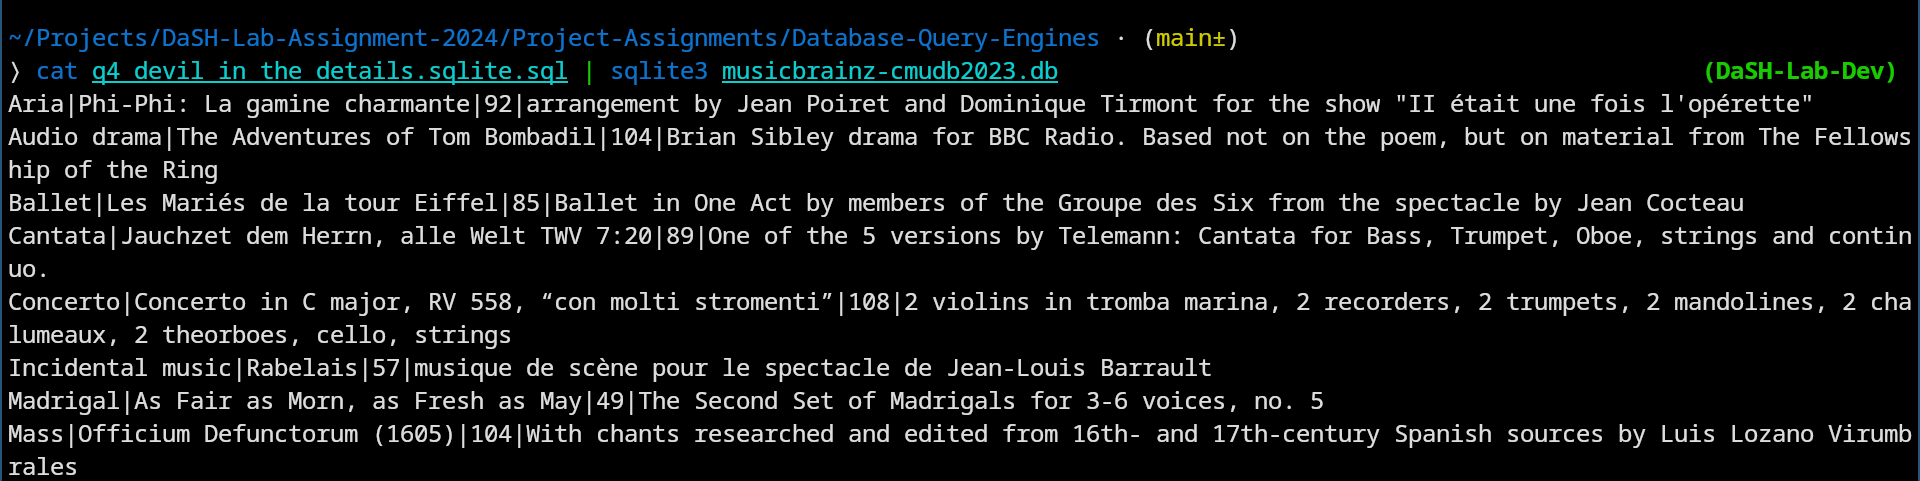
\includegraphics[width=.9\linewidth]{./images/Q4.png}
\end{center}
\subsection{Q5 - Find the artist with top releases for each month.}
\label{sec:orgd42319f}
\subsubsection{Query}
\label{sec:org4acb040}
\begin{verbatim}
 SELECT
    a.name AS artist_name,
    ri.date_month,
    COUNT(r.id) AS release_count
FROM
    artist a
JOIN
    artist_credit ac ON a.id = ac.id
JOIN
    release r ON ac.id = r.artist_credit
JOIN
    release_info ri ON r.id = ri.release
WHERE
    a.name LIKE 'Elvis%'
    AND a.type = (SELECT id FROM artist_type WHERE name = 'Person')
    AND ri.date_month IS NOT NULL
GROUP BY
    a.id, a.name, ri.date_month
ORDER BY
    release_count DESC,
    a.name ASC,
    ri.date_month ASC;
\end{verbatim}
\subsubsection{Output}
\label{sec:orgd3ea563}
\begin{center}
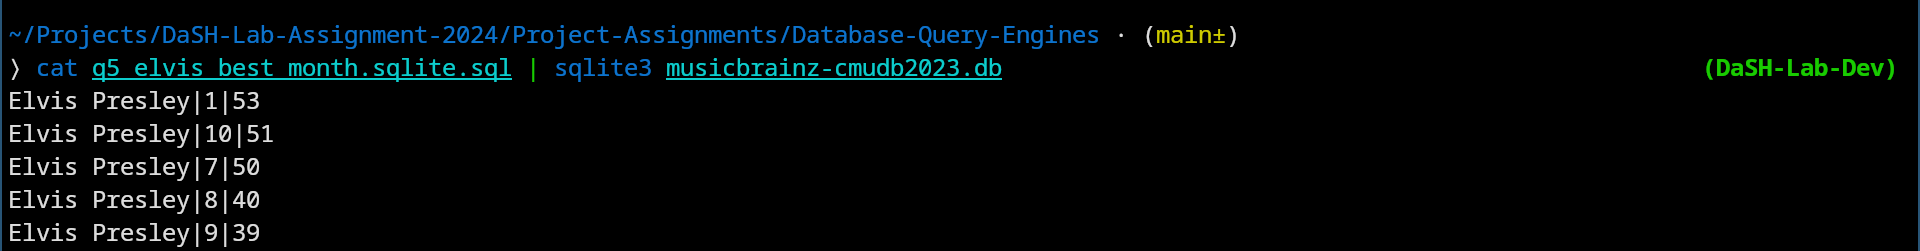
\includegraphics[width=.9\linewidth]{./images/Q5.png}
\end{center}
\subsection{Q6 - List the number of groups that were formed in the United States in each decades from 1900 to 2023.}
\label{sec:orgb62de75}
\subsubsection{Query}
\label{sec:org9bc3efa}
\begin{verbatim}
 SELECT
    CONCAT((begin_date_year / 10) * 10, 's') AS decade,
    COUNT(*) AS group_count
FROM
    artist a
JOIN
    area ar ON a.area = ar.id
WHERE
    ar.name = 'United States'
    AND a.type = (SELECT id FROM artist_type WHERE name = 'Group')
    AND begin_date_year BETWEEN 1900 AND 2023
GROUP BY
    (begin_date_year / 10) * 10
ORDER BY
    (begin_date_year / 10) * 10 ASC;
\end{verbatim}
\subsubsection{Output}
\label{sec:org2c404ba}
\begin{center}
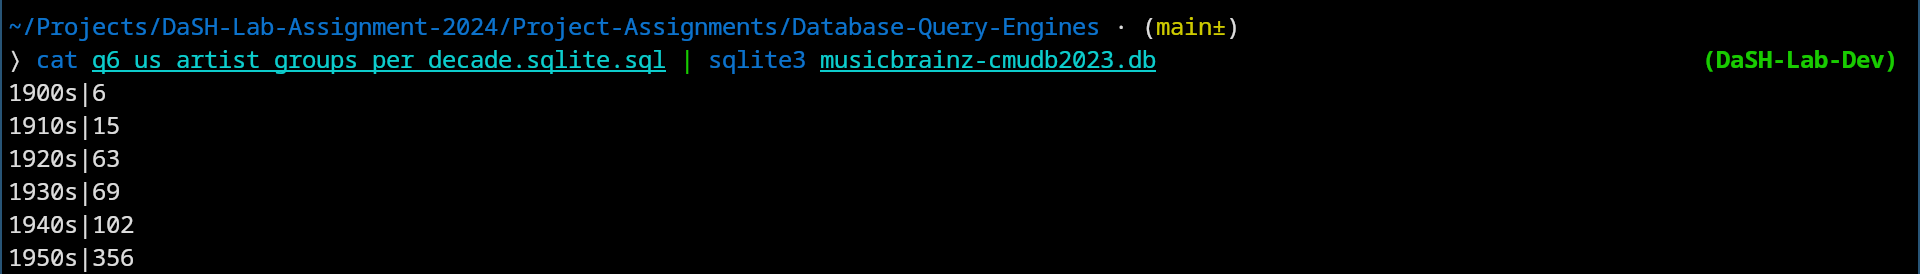
\includegraphics[width=.9\linewidth]{./images/Q6.png}
\end{center}
\subsection{Q7 - List all the artists who have collaborated with Pittsburgh Symphony Orchestra.}
\label{sec:orgf873dfc}
\subsubsection{Query}
\label{sec:orge774e28}
\begin{verbatim}
SELECT DISTINCT a.name
FROM artist_credit_name acn
JOIN artist a ON acn.artist = a.id
WHERE acn.artist_credit IN (
    SELECT ac.id
    FROM artist_credit ac
    JOIN artist_credit_name acn2 ON ac.id = acn2.artist_credit
    JOIN artist a2 ON acn2.artist = a2.id
    WHERE a2.name = 'Pittsburgh Symphony Orchestra'
)
AND a.name != 'Pittsburgh Symphony Orchestra'
ORDER BY a.name ASC;
\end{verbatim}
\subsubsection{Output}
\label{sec:org51481f2}
\begin{center}
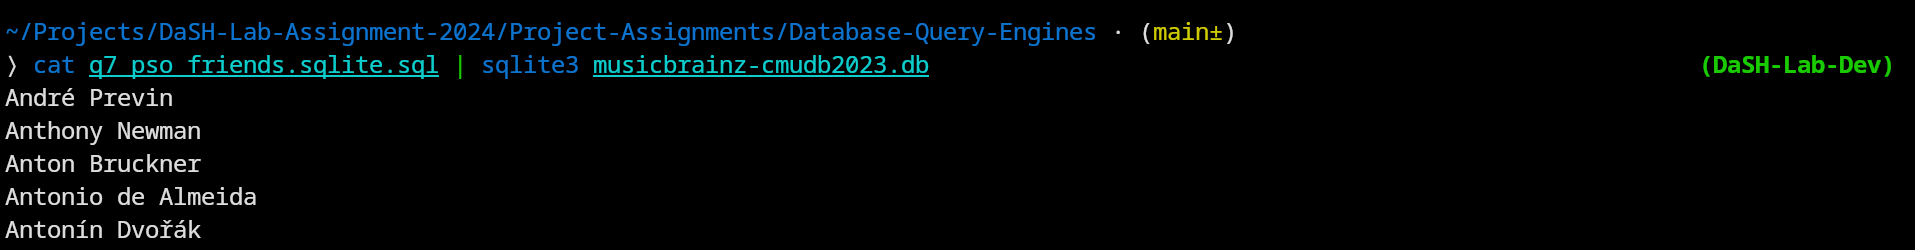
\includegraphics[width=.9\linewidth]{./images/Q7.png}
\end{center}
\end{document}
